Social marketing has been shown to much more effective than education in promoting pro-environental behavior \citep{mckenzie1999fostering}.  This further suggests that particular habits or existing structures outweigh the effect of new information.  The social marketing movement may be an important user of the results of the current project.  Recently, deliberative and inclusionary procedures (DIPS) has emerged as a powerful technique, which engages citizens in decision-making as a way to empower, inform, and transform constituents \citep{bloomfield1998deliberative}.  This is an exciting development which will nonetheless not be deeply engaged in this project.  Like other institutions, the expansion or contraction of the use of round tables and citizen juries typical of DIPS can be modeled based on existing data, and the model from this project will have the potential to identify them as strong action points.

However, unlike climate models where each cell's model is independent except at its boundaries, certain properties of the various elements of the model can be shared between all of the nodes that use it.  For example, a state's institution for monitoring water quality may influence many districts independently, but activities in each district draw from a single budget.

One property shared by each model component is its aggregate behavior.  For example, pollution levels in each district in a state combine to form that state's aggregate pollution stock.  Many of the same dynamics apply to pollution at both the district scale and the state scale, and the two values are related.  This relationship between scales of resolution motivates this project's goal to build self-similarity deeply into its model framework.  

Given that, there is little reason to simulate all regions simultaneously.  Instead, a single ``vertical'' slice of the network can be simulated, by assuming previously computed allotments of aggregate values for all of the other sub-regions.  This would result in a new data point, which then informs that sub-region's allotment probanility distribution function (which could be represented just as a mean and a variance).  Finally, some available data will represent ``output'' variables-- variables that are related to the selected allotments by equations that are not easily reversible.  Again, rather than using numerical analysis techniques to find solutions, which may themselves be distorted by inaccurate allotments, error terms will be calculated and used to weight the corresponding contribution to the sub-region's solution distribution.

% In fact, quality of life should be worst-off as highest-weighted
The World Commission on Environment and Development defined sustainable development as development that ``meets the needs of the present without compromising the ability of future generations to meet their own needs''.  A reasonable proxy for the first is the Quality-of-life index, and the Living Planet index can reflect the second (both calculated at the present time).  OLS models will be used to estimate global indices based on United States variables.  The total score, $S_{SD}$ for a run of the model then is,
\[
S_{SD} = \int_{t=now}^{\infty} I_{QoL}(t) I_{LP}(t) e^{t/\tau} dt
\]
integrated over all time of the simulation, where $I_{QoL}$ is the Quality-of-Life Index, and $I_{LP}$ is the Living Planet Index.  The exponential term reflects the decreasing confidence in the model's results, with time constant $\tau$.  Since the model cannot be run forever, the final slope of the $I_{QoL}$ and $I_{LP}$ indices can be used to approximate the total integral:
\[
\tilde{S}_{SD} = \int_{t=t_{now}}^{t_{end}} I_{QoL}(t) I_{LP}(t) e^{t/\tau} dt + e^{-t_{end}/\tau} \left(\tau^2 \frac{d I_{QoL} I_{LP}}{dt}(t_{end}) + \tau I_{QoL}(t_{end}) I_{LP}(t_{end})\right)
\]

% Write equations here, showing X-bar for each sub-region and each point in time, being a normal distribution, and then X-bar for this sub-region initially being set as a random point in whatever is left over, and then being changed in each timestep by a probabilistic difference based on the changes in other's allotments

  \item How to ensure that incomplete models do not distort dynamics?  The model will evolve over time as more institutions are added.  When a relevant institution is entirely missing, but its effect are reflected in the aggregate data, the model must ``fail gracefully'', either by distorting results only at the institutional level, or by inferring the existence of unrepresented variables if the existing dynamics cannot account for them.

    From the 'perspective' of a node on one of the networks, the model looks like a system dynamics model with additional constraints which come from the other networks in which the components play a part.  From the perspective of a particular model component, the model is the collection of node-systems in which it plays a role-- both the vertical hierarchy of scale networks (regional vs. subregional) and institutional networks.  A further perspective could be focus on the system dynamics model, which may change from one region to another, but on a deep level those parts of it that do not change represent the same system even though they act on different contexts.

The techniques of Dynamic Network Analysis may be applicable for this process \citep{carley2003dynamic}.

@conference{carley2003dynamic,
  title={{Dynamic network analysis}},
  author={Carley, K.M.},
  booktitle={Dynamic social network modeling and analysis: Workshop summary and papers},
  pages={133--145},
  year={2003}
}

miller2006recruiting

@conference{miller2006recruiting,
  title={{Recruiting clients to a community-based HIV-prevention program: A dynamic model}},
  author={Miller, R.L. and Levine, R. and Khamarko, K. and Valenti, M.T. and McNall, M.A.},
  booktitle={Proceedings of the 24th international conference of the system dynamics society conference. Nijmegen, Netherlands},
  year={2006}
}

The earliest models presumed that the problem was a lack of information, but these models proved to be incomplete.  Other authors have tried to look for the role of common-sense variables in determining pro-environmental behavior, such as rationality, competitive orientation, values, and satisfaction of needs, but these have had mixed results.

However, the large number of proposed variables found to be poor predictors of actual behavior suggest the need for a model where inclusion of a variable does not necessitate their use.

\begin{quotation}
One of the most important insights which the social scientist can offer in the environmental debate is that the eminently rational appeals on the part of environmentalists for 'us' to change our attitudes, or lifestyles, so as to advance a general 'human interest' are liable to be ineffective.
\end{quotation}

\begin{figure}[htb]
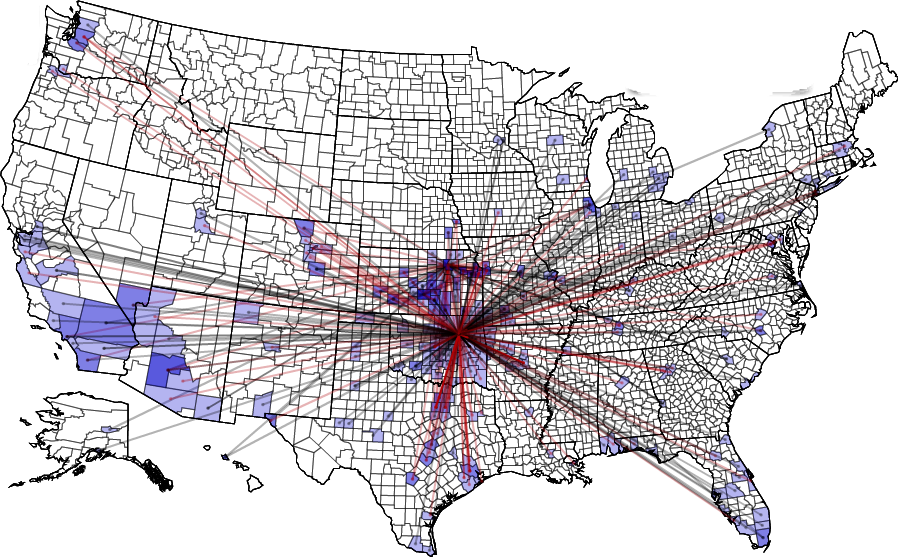
\includegraphics[width=6in]{districtnetwork2.png}
% Drop this figure?  Just mention the possibilities?
\caption{Example district network, for three counties (Riley County, Kansas, Reno County, Kansas, and Tulsa County, Oklahoma), based on migration patterns.  {\footnotesize Data Source: Internal Revenue Service, inter-county moves of 10 or more people.  Modified from: Jon Bruner, Map: Where Americans Are Moving, Forbes.com: {\tt http://www.forbes.com/2010/06/04/migration-moving-wealthy-interactive-counties-map.html}}}
\end{figure}

@book{ajzen1980understanding,
	Author = {Ajzen, I. and Fishbein, M. and Heilbroner, R.L.},
	Publisher = {Prentice-Hall Englewood Cliffs, NJ},
	Title = {{Understanding attitudes and predicting social behavior}},
	Year = {1980}}


 (such as the agency model described by \citet{ajzen1980understanding}) 

Even large models, like the System Dynamics National Model, have been influenced by this trend.  The National Model originally was proposed as including several economic sectors, but these were collapsed into just two, capital plant and consumer goods, for the purpose of clarity \citep{Forrester1991}.

  Instead, a combination of peer review of its components and computational analyses are needed to validate it and to abstract relevant subsections.  A discussion of the proposed size for this model is included in section \ref{sec:implementing}.

  In many cases, data series are only available at one scale-- such as the nation-wide scale-- but similar dynamics (that is, self-similar models) apply to all scales. 

small-world relationships can be embedded into the network graphs upon which the dynamics are modeled.  Scale-free behavior is implicitly assumed, unless explicitly modified, as models are duplicated on smaller levels.  The hierarchies in society are represented as hierarchies of networks, at national, state, and metropolitan levels.  

By capturing the relationships between constitutive elements, in such a way that present dynamics can be reproduced, the model can serve as a guide for identifying leverage points.  However, unlike many system dynamic models, that guide is not primarily intended for human audiences or direct education.  

  Networks need not represent spacial distinctions: demographics and corporate relations can also be encoded as networks, easing the need to reproduce dynamics across the different groups.  The framework will allow each region or institution to be represented by multiple maps, and elements within each partial model to play roles in multiple coexisting networks.

the process of applying self-similar dynamics to regional models, by either determining parameter values (as with GIS data), or providing a baseline against which the results of stochastic allotments are measured (see \ref{fig:trialestimate}).

 (for example, either as a distinct policy change one dynamic to another, or as weighted combination of both).

  \item What existing models could form the starting point for the national dynamics, and upon what criteria should one be selected?  The World3/2000 model, the MIT System Dynamics Group's National Model, the Department of Energy's National Energy Modeling System, and the Redefining Prosperity Project's LowGrow model each have attractive features.
% How are different models to be combined?

The use of self-similarity greatly facilitates identifying leverage points, but it remains a daunting proposition.  A model on the order of the National Model would capture many of the important dynamics that drive climate change, and combining this with self-similar networking and regional data would allow one to identify particular regions that might act as linchpins in the climate system.  System dynamic modeling software is typically very fast, but benchmarks are not available.
